\documentclass[a4paper]{article}
\usepackage{forest}
\usepackage{float}
\usepackage{geometry}
\usepackage{listings}
\usepackage{hyperref}
\usepackage{graphicx}
\usepackage{ragged2e}
\usepackage{color}
\usepackage{xepersian}
\usepackage{subfiles}
\newgeometry{left=1.4cm, right=1.4cm, bottom=2.0cm, top=2.0cm}
\settextfont[Scale=1]{XB Roya}

\renewcommand{\baselinestretch}{1.5}
\definecolor{dkgreen}{rgb}{0,0.6,0}
\definecolor{gray}{rgb}{0.5,0.5,0.5}
\definecolor{mauve}{rgb}{0.58,0,0.82}
\definecolor{commentColor}{rgb}{0.6,0.6,0.60}

\title{معماری مقیاس بزرگ \\ خانم دکتر سحر آدابی}
\author{علیرضا سلطانی نشان}

\begin{document}
\maketitle
\tableofcontents

\section*{مجوز}

به فایل license همراه این برگه توجه کنید. این برگه تحت مجوز GPLv3 منتشر شده است
که اجازه نشر و استفاده (کد و خروجی/pdf) را رایگان می‌دهد.

\section{پیشگفتار}

اگر درس مهندسی نیازمندی‌ها را خوانده باشید، احتمالاً در جریان آن هستید که برای
تولید نرم‌افزار بخش‌های زیادی درگیر هستند اما در حالت کلی در درس پیشین دانستیم
که در ابتدا بایستی نیازمندی‌های مشتری یا کارفرما را از محصول نرم‌افزار بدانیم،
آن را بررسی و تحلیل کنیم، سند نیازمندی آن را آماده‌سازی کنیم و سپس به دنبال
طراحی معماری آن برویم. در این درس به طراحی و پیاده‌سازی سند معماری مقیاس بزرگ یک
محصول نرم‌افزاری می‌پردازیم تا فرایند تولید نرم‌افزار را به طور کامل طی کرده
باشیم.

\section{معرفی}

\subsection{چه زمانی یک پروژه مقیاس بزرگ است؟}

برای اینکه بتوانیم بگوییم که چه پروژه‌ای مقایس بزرگ محسوب می‌شود، براساس دو
استاندارد ایرانی و بین‌المللی می‌توان دو استاندارد را در اینجا مطرح کرد:

\begin{itemize}
    \item استاندارد مقیاس بزرگ بودن پروژه از نظر دکتر شمس، آن است که پروژه بیشتر
    از ۶ ماه زمان پیا‌ده‌سازی نیاز داشته باشد و تعداد درخواست‌های ارسالی به آن
    ۱۲ نفر به بالا باشد.
    \item استاندارد بین‌المللی مقیاس بزرگ بودن پروژه را زمان یک سال به بالا جهت
    پیاده‌سازی و تعداد درخواست‌ها را بین ۲۰ تا ۲۲ نفر تعیین می‌کند.
\end{itemize}

ابتدایی ترین فاز معماری یک محصول نرم‌افزاری مقیاس بزرگ، طراحی و بررسی و آنالیز
سناریو‌های آن است.

سند معماری نرم‌افزار به مجموعه‌ای از سناریو‌هایی گفته می‌شود که در ازای هر کدام
یک راه‌حل مناسب مطرح می‌شود.

یکی از نیازمندی‌های بررسی معماری نرم‌افزار مقیاس بزرگ استفاده از متدولوژی
\lr{RUP}\footnote{\lr{Rational Unified Process}} می‌باشد. دلیل اصلی آن این است
که می‌توان تمام فرایند‌های آن را به همراه \lr{Artifact}ها شخصی‌سازی کرد. در
معماری نرم‌افزار می‌توانیم مشخص کنیم که چه اجزایی داریم و این اجزا چگونه با
یکدیگر در ارتباط هستند و شامل چه قید‌هایی می‌شود. در حقیقت در سند معماری
نرم‌افزار نمود خارجی المان‌ها را مطرح می‌کنیم. نحوه در کنار هم چیدن سرویس‌ها را
مطرح می‌کنیم اما هیچ وقت در مورد جزئیات اینکه برای مثال از چه الگوریتم‌هایی
استفاده می‌کنیم، صحبت نمی‌شود. در این سند علاوه‌بر نیاز‌های جاری، در مورد
نیاز‌های آتی نیز صحبت می‌شود که در آینده چقدر باید نرم‌افزار قابلیت گسترش
\lr{Expandability} داشته باشد.

\subsection{یادآوری متدولوژوی \lr{RUP}}

این متدولوژوی به عنوان یک متدولوژوی توسعه نرم‌افزار اجایل، به دلیل قابل تکرار
بودنش در نظر گرفته شده است. این روش مهندسی نرم‌افزار از یک سیستم انعطاف پذیر و
سازگار در فرایند توسعه نرم‌افزار استفاده می‌کند که در برگیرنده انجام تنظیمات و
تکرار دوره‌های مهندسی نرم‌افزار است تا زمانی که محصول به نیازمندی‌های مطرح شده و
اهداف برسد \cite{rupStudy}.

\subsubsection{منظور از نظم در \lr{RUP}}

منظور از نظم در حقیقت نمود‌هایی می‌باشد که در فرایند توسعه نرم‌افزار مورد
استفاده قرار می‌گیرد، در حقیقت نظم، مدل‌سازی حرفه‌ای را نشان می‌دهد. این نظم‌ها
به ما کمک می‌کنند که چه زمانی چه \lr{Activity}هایی را باید به چه میزان در چه
بازه‌هایی انجام دهیم و خروجی مورد نظر ما چیست؟

برای مثال در فرایند تحلیل نیازمندی پروژه، نظم نیازمندی، خروجی فاز‌های آن است که
به شکل مدل‌های \lr{Usecase diagram} و سند معماری نرم‌افزار کشیده و نوشته شده
است.

\subsubsection{چهار فاز اصلی در \lr{RUP}}

\begin{enumerate}
    \item فاز آغاز یا \lr{Inception}: در این فاز تمام نیازمندی‌ها جمع‌آوری
    می‌شود و مقیاس پروژه در آن بدست می‌آید.
    \item فاز توسعه یا \lr{Elaboration}: طراحی سیستم و تحلیل دقیق‌تر نیازمندی‌ها
    صورت می‌گیرد.
    \begin{enumerate}
        \item استفاده از مدل‌سازی‌ها و کشیدن دیاگرام‌ها
        \item کشیدن مدل \lr{usecase}: کاربرد بزرگی برای مشتری (کارفرما) و طراح
        دارد و برای هر دو طرف قابل فهم می‌باشد. در این نوع نمودار افعال و
        نیازمندی‌های \lr{functional} مطرح می‌شود. انتظارات در مورد سیستم در
        اینجا مورد بحث قرار می‌گیرند.
        \begin{itemize}
            \item اینکه کاربرد بتواند زیر ۲ ثانیه احراز هویت شود مربوط به
            نیازمندی‌های \lr{non-functional} می‌باشد.
            \item شامل دو سند می‌شود:
            \begin{itemize}
                \item سند \lr{Usecase} که انتظارات سیستم را مشخص می‌کند.
                \item سند معماری که \lr{function} و \lr{non-functional} را در بر
                می‌گیرد.
            \end{itemize}
        \end{itemize}
        \item طراحی \lr{Class diagram} 
        \item طراحی \lr{Sequence diagram}
    \end{enumerate}
    \item فاز ساخت یا \lr{Construction}: در این فاز کد نویسی و ارزیابی کد‌های
    نوشته شده صورت می‌گیرد.
    \item فاز استقرار یا \lr{Deployment}: در این فاز نرم‌افزار آماده شده است و
    در بستری مناسب به کاربران نهایی \footnote{\lr{End users}} ارائه می‌شود که
    نیازمند آموزش‌های لازم می‌باشد.
\end{enumerate}

محبوبیت استفاده از متدولوژی \lr{RUP} به خاطر آن است که کاملاً به صورت جامع سیستم
را در بر می‌گیرد.

\subsubsection{منظور از فرسخ‌شمار چیست؟}

فرسخ‌شمار یا \lr{Milestone} در هر کدام از فاز‌ها مشخص می‌شود که در حقیقت در مورد
تعیین یک بازه زمانی مشخص صحبت می‌کند. در آن می‌توانیم ببینیم که در فاز‌های قبلی
چه کار‌هایی بایستی انجام می‌شده، آیا آن‌ها را انجام داده‌ایم و اگر انجام
نداده‌ایم یا مشکلی در آن وجود دارد آن فاز را تکرار می‌کنیم تا به انتهای آن برسیم
که به نحوی تسک یا وظیفه را ببندیم.

\subsubsection*{نکات}

\begin{itemize}
    \item ساده‌ترین سند در میان این ۴ فاز، سند استقرار می‌باشد.
    \item معماری مقیاس‌پذیر (بزرگ) یک پروژه نرم‌افزار دو بُعد پویا و ثابت دارد.
    \item در مورد ارزیابی کارایی و آزمون نرم‌افزار گفتنی است که هر توسعه‌دهنده
    مسئول \lr{Quality control} بخش خودش است.
    \item تکرار‌ها \lr{n} تا هستند مدیر پروژه یا طراح سیستم باید به ما تعداد
    تکرار‌ها را به صورت تقریبی بگوید.
\end{itemize}

\subsubsection{محوریت بر روی نیازمندی‌ها}

متدولوژوی \lr{RUP} تاکید زیادی روی شناسایی و مدیریت نیازمندی‌ها را دارد و به
تیم‌ها کمک می‌‌کند تا نیازمندی‌های کلیدی پروژه‌ را به خوبی درک و پیاده‌سازی
کنند.

\subsubsection{استفاده از برنامه‌نویسی \lr{OOP}}

این متدولوژی به طور گسترده از ۴ اصل شیء‌گرایی استفاده می‌کند و به توسعه‌دهندگان
اجازه می‌دهد که کد‌های قابل استفاده مجدد و مدیریت فاکتور‌های انعطاف پذیری را
ایجاد کنند.

\section{معماری مقیاس بزرگ نرم‌افزار}

\subsection{معماری نرم‌افزار چیست؟}

معماری نرم‌افزار یک تعریف واحد ندارد. معماری نرم‌افزار یک برنامه یا یک سیستم
محاسباتی می‌باشد. یک ساختار یا مجموعه ساختار‌هایی است از سیستم مورد نظر ما که
متشکل از المان‌های کامپیوتری است و نمود خارجی یک چیز (المان) می‌باشد و ارتباطات
بین آن‌ها را در بر می‌گیرد. هیچ‌گاه نمی‌توان نرم‌افزاری نوشت که معماری نرم‌افزار
نداشته باشد. برای مثال از معماری \lr{MVC} در نرم‌افزار خود استفاده کرده‌ایم.
نرم‌افزاری وجود ندارد که معماری نداشته باشد. اگر بگوییم نرم‌افزاری معماری ندارد
در حقیقت علم معماری به کار گرفته شده را نمی‌دانیم که آن را بی‌معماری می‌نامیم.
برای مثال معماری کلاینت سرور که براساس نیازمندی‌های نرم‌افزاری بیان می‌شود که چه
بخش‌هایی سمت سرور باشد چه‌ بخش‌هایی سمت کلاینت.

\subsection{معمار نرم‌افزار کیست؟}

معمار نرم‌افزار شخصی مدبر است که تجربه تخصصی آن در حوزه‌ای مشخص بیشتر از ۱۰ سال
است که تسلط کافی در آن سیستم مشخص دارد و از ابتدا تا انتهای پروژه با فرایند
توسعه و توسعه‌دهندگان همراه است.

\subsection{المان‌ها}

بخش‌های یک سیستم نرم‌افزاری را گویند برای مثال یک نرم‌افزار واحد مانیتورینگ،
واحد زمان‌بندی، واحد بررسی درخواست‌ها و غیره را دارد.

\subsection{\lr{External Feasible Properties}}

آن بخش چه وظیفه‌ای را باید انجام دهد و آن بخش آن وظیفه را در حال انجام است یا
خیر؟ جزئیات مربوط به المان‌های درگیر در بخش معماری در \lr{External Feasible
Properties} مطرح نمی‌شود.

\subsection{تفاوت کامپوننت و المان}

وقتی در مورد کامپوننت می‌گوییم در حقیقت چیزی است که می‌خواهیم آن را پیاده‌سازی
کنیم. المان کامپوننتی است که قسمت اجرایی را برای آن در نظر نگرفته‌ایم.

\subsection{بخش‌هایی که معماری نرم‌افزار باید پوشش دهد}

\begin{enumerate}
    \item المان‌هایی که در سیستم قرار است استفاده شود را مشخص می‌کند.
    \item نمود خارجی المان‌های سیستم مورد نظر را مشخص می‌کند و تعیین می‌کند هر
    المانی در سیستم چه وظیفه‌ای را انجام دهد.
    \item ارتباطات بین المان‌ها را به روشنی مشخص می‌کند.
\end{enumerate}

در کنار تمامی موارد بالا، بخش‌هایی که یک معماری نرم‌افزار پوشش نمی‌دهد شامل ذات
المان‌ها می‌باشد.

\subsection{قابلیت اطمینان یا \lr{Reliability}}

یک سیستمی که در زمان مشخص درست کار کند به شرطی که در زمان $T - x$ درست کار کرده
باشد.

\subsection{قابلیت استفاده یا \lr{Useability}}

سیستمی که کارآمد باشد برای آن دسته از افرادی که سیستم را حاضر و آماده کرده‌ایم.
به گونه‌ای که با ظاهر مناسب کار کردن با آن نیز آسان باشد.

\subsection{ارائه سریع محصول یا \lr{Short time to market}}

قابلیت یا \lr{Feature} مجموعه‌ای از توابع نرم‌افزاری است که وقتی در بازار ارائه
می‌شود، واقعاً کار می‌کند. 

\subsubsection*{نکات}

\begin{itemize}
    \item تا آنجایی که می‌شود هزینه‌ها را باید کاهش بدهیم و بیشترین هزینه‌ها را
    ما در بخش توسعه نرم‌افزار خواهیم داشت. همیشه باید کارمندان را مشغول توسعه
    نگهداریم تا باعث از دست رفتن هزینه‌ها نشود.
    \item مشکل معمار آن است که حجم زیادی از نیازمندی‌های نرم‌افزاری را در حال
    بررسی است که نسبت به هم در تضاد هستند.
    \item بخشی از وظایف اصلی معماری نرم‌افزار مشخص کردن استک‌های نرم‌افزاری
    می‌باشد. بخش دیگری از آن این است که بررسی کند این موارد توسط تیم اجرا و
    استفاده می‌شود یا خیر (\lr{Follow up})
\end{itemize}

\subsection{تفاوت معماری سازمانی و معماری نرم‌افزار}

معماری سازمانی و معماری نرم‌افزار با یکدیگر متفاوت است. در معماری سازمانی، چارت
سازمانی آن مشخص‌کننده محدوده و کلیت هر قسمت آن سازمان می‌باشد.

% \lr{Mobile Adhoc Network}

% شبکه‌های موردی متحرک

% یک شبکه‌ای است فاقد زیرساخت. بیشتر در مناطق جنگی و \lr{Real-time} مورد استفاده
% قرار می‌گیرد که بتوانیم در حال حاضر یک شبکه را آماده کنیم که سربازان با یکدیگر
% ارتباط بگیرند به گونه‌ای که \lr{Mobility} بیان می‌کند که شبکه را بایستی با
% زیرساخت مناسب ایجاد کند.

% یک پیام «سلام» ارسال می‌کند و منتظر دریافت \lr{ACK} می‌باشد و بعد از آن سعی
% می‌کند که ارتباط را حفظ کند تا آن کانال ارتباطی بین سربازان برقرار باشد.

\subsection{جزئیات فعالیت‌های معماری نرم‌افزار}

\subsubsection{ساخت \lr{Business case} برای سیستم}

\subsubsection*{یادآوری \lr{Business plan}}
بیزینس پلن سندی است که چهارچوب سیستم ما را در بر می‌گیرد و آن را نسبت به سیستم
مشابه مقایسه می‌کند و آن را به چالش می‌کشد. نسبت به هر چالشی که در سیستم ما وجود
دارد بایستی پاسخی مطرح شده باشد.

سند \lr{Business case} سندی از جنس مالی است که در آن برآورد هزینه و توجیهات
اقتصادی بیان شده است. در این سند، درگیر بودن نیرو‌ها بررسی می‌شود و در نهایت
توجیهات‌ اقتصادی را از نظر کاهش هزینه‌ها مطرح می‌کند. برای مثال ممکن است بیشتر
اوقات بهره‌وری سیستم را افزایش داده باشیم که نسبت به این افزایش باید توجیهی وجود
داشته باشد.

از ابتدا تا انتهای پروژه دائماً در حال تخمین قیمت پروژه به عنوان معمار نرم‌افزار
هستیم که در آن هزینه‌ای را مطرح می‌کنیم که بررسی کرده‌ایم در توسعه نرم‌افزار
نیاز خواهد شد. در این حین اگر هزینه توسعه بیشتر شود باعث ضرر ما و اگر کمتر شود
باعث سود ما خواهد شد. پس به همین دلیل سعی می‌کنیم سند \lr{Business case} را از
ابتدا تا انتهای فرایند پروژه توسعه دهیم و توجیه اقتصادی به روزی در آن داشته
باشیم که موجب ضرر از سمت پیمانکار نشود.

\subsubsection*{نقطه سر به سر یا \lr{Break event point}}

وضعیتی است که در آن هزینه‌هایی که ما برآورد کرده‌ایم در بازه زمانی مشخص، برابر
با صفر شده است. برای مثال اگر مبلغ ۵۰۰ میلیون تومان را به عنوان هزینه نرم‌افزار
محاسبه کرده باشیم و طی یک سال دیگر سازمان دقیقاً همان مبلغ را بدون کاهش یا
افزایش پرداخت می‌کند این وضعیت نقطه سر به سر خواهد شد. زمان نقطه سر به سر
معمولاً در بازه ۲ تا ۵ سال تعریف می‌شود که در واقعیت زمان خیلی طولانی برای تخمین
هزینه توسعه نرم‌افزار محسوب می‌شود.

\subsubsection{فهمیدن نیازمندی‌های پروژه}

نیازمندی‌ها تنها متغیر ثابت هستند. همانطور که پیش‌تر اشاره شد
\lr{non-functional}ها در قالب سند معماری نرم‌افزار دیده می‌شوند. همچنین اگر
نیازمندی \lr{functional} وجود نداشته باشد \lr{non-function}ها معنایی ندارند.
برای مثال می‌گوییم که نرم‌افزارمان بایستی امن باشد، یعنی \lr{Usecase diagram}
داریم که ازای آن نیازمندی \lr{non-function} تعریف کرده‌ایم.

نکته مهم آن است که مهمار نرم‌افزار تنها نیازمندی‌های جاری را در نظر نمی‌گیرد
بلکه نیازمندی‌های آتی را هم در سند پیشبینی می‌کند تا بتواند یک جریان را کامل کند
و به نوعی \lr{Proof of concept} داشته باشد.

\subsubsection{ایجاد یا انتخاب یک معماری نرم‌افزار}

معمار نرم‌افزار معمولاً یا یک معماری را انتخاب می‌کند یا آن را از نو می‌سازد.
ممکن است در تز‌های آکادمیک معماری جدیدی را ایجاد کرده باشیم زیرا ممکن است صورت
مسئله‌های جدیدی پدید آمده باشند یا نیازمندی‌های \lr{non-function} جدیدی یافت شده
باشد. در حالت کلی معماری‌ها را یا باید بهینه‌سازی کنیم یا اجرا و در پروژه
نرم‌افزاری پیاده کنیم.

\subsubsection{دنبال کردن معماری یا \lr{Communicating the architecture}}

چیزی که در معماری نرم‌افزار بیان شده است را دنبال کنیم و بررسی کنیم که تمام آن
فرایند‌های مهندسی توسعه نرم‌افزار را توسعه‌دهنده‌ای دنبال می‌کند یا خیر. بیان
این مسئله طرف معمار و اجرای آن در طرفی دیگر است. خیلی با بخش \lr{Implementing
based on the architecture} ارتباط دارد.

\subsubsection{بررسی و ارزیابی معماری}

نکته مهم آن است که در حوزه معماری نرم‌افزار چیزی به نام شبیه‌سازی نداریم چرا که
قدم ابتدایی هر پروژه‌ای تعیین معماری آن است. اینکه از ما سوال شود که معماری
نرم‌افزارتان را با چه شبیه‌سازی اجرا کردین یا با چه فاکتور‌های شبیه‌سازی آن را
ارزیابی کرده‌اید، بحث کاملاً غلطی می‌باشد. مقایسه بین الگوریتم‌ها امکان‌پذیر
می‌باشد زیرا داریم شبیه‌سازی ورکلود‌ها را انجام می‌دهیم.

در این خصوص روشی را داریم به نام \lr{ATAM} که ارزیابی معماری نرم‌افزار را
می‌توان از طریق آن انجام داد. یک استاندارد مشابه با \lr{ISO} می‌ماند که
نیازمندی‌های \lr{non-functional} را در نظر می‌گیرد. یک تیم مستقل با آن همراه است
که بررسی کند ما از راه درستی استفاده کرده‌ایم یا خیر. در نهایت به ما نشان می‌دهد
که نسبت به آن سناریو می‌توانیم این معماری را پوشش دهیم یا خیر.

برای بررسی و ارزیابی معماری راه‌های مختلفی وجود دارد:

\begin{enumerate}
    \item مدل‌سازی صوری، فرمال و رسمی: برای اینکه ثابت کنیم چیزی که داریم
    می‌نویسم قابل تایید است و درست می‌باشد. به دلیل آن که ریاضی هستند می‌توانند
    مفید و رویکردی مناسب باشند.
    \item استفاده از \lr{ADL: Architecture Definition Language}
    \item استفاده از \lr{Prototype}ها: اگر یک سیستم کوچک درست کنیم که به
    صورت صحیح کار کند می‌تواند نشان دهنده آن باشد که سیستم اگر بزرگتر شود هم
    صحیح کار خواهد کرد.
    \item ۸۰ درصد نیازمندی‌ها و دامنه‌های مسئله با نرم‌افزاری که در حال کار است
    که با این معماری انطباق دارد پس قطعاً معماری با کار‌های آینده ما نیز منطبق
    خواهد بود.
\end{enumerate}

\subsubsection*{نکته}

دامنه مسئله مثل دامنه سیستم‌های مالی، دامنه سیستم‌های آموزشی و غیره یک تعریف
مسئله مخصوص و واحد دارد که در سیستم‌های گوناگون مشابه یکدیگر هستند و دقیقاً
نیازمندی‌های آن‌ها نیز مشابه هستند. اگر یک سیستم مشابه را پیدا کردیم، معماری
انتخابی ما می‌تواند با سیستم مشابه نیز کار کند.

\subsubsection{پیاده‌سازی مبتنی بر معماری}

بررسی اینکه آیا تمام فرایند‌هایی که در فاز‌های توسعه نرم‌افزار شروع می‌شود با
بیانات و نقشه‌راه معمار نرم‌افزار مطابقت دارد یا خیر؟

\subsubsection{اطمینان از انطباق نسبت به یک معماری}

در این بخش بررسی می‌کنیم که فرایند‌ها تماماً تابعی از معماری هستند یا خیر؟ در
انتهای کار، تمام‌ اسناد را در کنار هم قرار می‌دهیم و به تطبیق اسناد با سند
معماری می‌پردازیم. برای مثال تمام \lr{Usecase diagram}ها مطابق با سند معمعاری
\lr{Usecase}ها بوده‌اند؟ طبق استاندارد طراحی شده‌اند؟ اگر هر کدام مطابقت نداشت
بایستی سریعاً اصلاح شود تا از ایجاد هزینه‌های آینده جلوگیری به عمل آورد. ما
بایستی مطمئن باشیم که تمام اسنادی که به معمار نرم‌افزار تحویل می‌دهیم مطابق با
سند معماری باشد که شامل چندین بخش خواهد شد.

\subsection{چه چیزی یک معماری خوب را تحویل می‌دهد؟}

هیچ چیز ذاتاً خوب یا بد نیست بلکه واسبتگی بسیار زیادی به کاربرد آن در سیستم مورد
نظر دارد. معماری کنترل دمای یک نیروگاه تولید برق را نمی‌توان در کنترل دمای خانه
استفاده کرد چون استفاده نادرست و نا به جایی بوده است. ذاتاً نمی‌توانیم بگوییم که
کدام معماری خوب است کدام معماری بد بلکه انتخاب ما نسبت به سیستم خوب و بد دارد.

معماری قابل ارزیابی است پس باید براساس اهدافی که داریم فرایند ارزیابی را انجام
دهیم تا در نهایت ببینیم که این ارزیابی چقدر می‌تواند معماری را با اهداف ما
\lr{Match} کند. برای مثال ممکن نیست که یک سامانه‌ای که امنیت ندارد را الهام
بگیریم برای سامانه‌ای که یکی از اهداف اصلی آن امنیت است.

نمودار زیر را از معماری سطح بالای \lr{ATM} را در نظر بگیرید:

\begin{figure}[H]
    \centering
    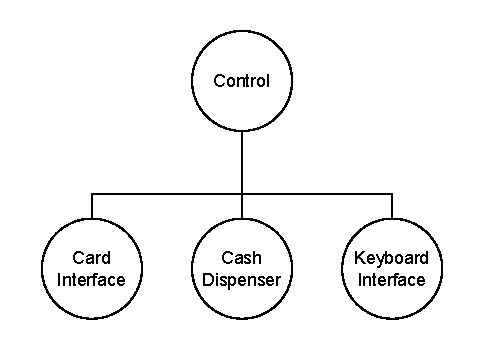
\includegraphics[width=0.5\textwidth]{images/bad-arch-of-atm.drawio.pdf}
    \caption{نمایش معماری سطح بالا دستگاه \lr{ATM}}
    \label{fig:atmDiagram}
\end{figure}

شکل شماره \ref{fig:atmDiagram} ساختار کلی از دستگاه \lr{ATM} را نمایش می‌دهد.
درست است که در مطالب بالاتر گفتیم که معماری یک چکیده از ساختار سیستم می‌باشد اما
در این نمودار ارتباطات بین المان‌ها کاملاً همراه با ابهام می‌باشد و تمام معماری
دستگاه \lr{ATM} را پوشش نمی‌دهد. در این نمودار ذات المان‌ها مشخص نیست. برای مثال
مشخص نیست که واحد \lr{Card interface} ممکن است هم کارت را دریافت کند هم اعتبار
کارت ورودی را بسنجد؟ پس می‌توان گفت وظیفه المان \lr{Card interface} در این
نمودار اصلاً مشخص نیست و در این نمودار دقیقاً ماهیت ارتباطات بین المان‌ها مشخص
نیست. همچنین لایه‌بندی در این نمودار به صورت واضح کشیده نشده است. در لایه‌بندی
همواره منطق وجود دارد مانند لایه‌بندی استاندارد \lr{OSI} که جانمایی المان‌ها در
این نمودار کامل کشیده نشده است. برای مثال بحث امنیت و کارایی و تعامل‌پذیری اصلاً
وجود ندارد. لایه‌بندی یک معماری تماماً توسط معمار نرم‌افزار مشخص خواهد شد.

\subsection{تفاوت \lr{Fault} با \lr{Failure}}

\lr{Fault} یعنی یک نقضی بالقوه در سیستم وجود دارد تا زمانی که سیستم بدون مشکل
کار کند آن نقض خودش را نمایان نمی‌کند اما در شرایط خاصی ممکن است برنامه به این
\lr{Falut} برخورد کند و بالفعل موجب از کار افتادن نرم‌افزار شود. در حقیقت بعد از
برخورد نرم‌افزار با \lr{Fault} پدیده‌ای به نام \lr{Failure} رخ می‌دهد. در حقیقت
\lr{Fault} در نرم‌افزار وجود داشته است که در شرایط خاص با ورودی خاص کاربر برنامه
با شکست یا \lr{Failure} رو به رو می‌شود و باعث کار نکردن درست نرم‌افزار خواهد
شد.

همواره \lr{Fault} از سمت طراحی نرم‌افزار همراه خواهد بود زیرا بایستی در اسناد
طراحی به آن نگاه مهندسی شود. زمانی که پیاده‌سازی می‌شود اگر در شرایط آزمون
بتوانیم آن \lr{Fault}ها را شناسایی کنیم و آن‌ها را رفع کنیم سیستم را از
\lr{Failure}های آینده نجات خواهیم داد.

نکته: \lr{Fault} موجب \lr{Failure} می‌شود.

اگر ما یک حافظه \lr{USB} داشته باشیم و در هنگام انتقال اطلاعات ناگهانی فلش را از
سیستم خارج کنیم، در حقیقت نه \lr{Fault} نه \lr{Failure} و نه \lr{Error} رخ داده
است. بلکه سیستم توسط عامل خارجی دستکاری شده است. اگر \lr{Fault} در سیستم داشته
باشیم بایستی توانایی هندل کردن آن را در نرم‌افزار داشته باشیم.

\subsection*{نکات}

\begin{itemize}
    \item معماری نرم‌افزار المان‌های نرم‌افزاری را مشخص می‌کند.
    \item \lr{Mapping} تسک‌ها به منبع مشخص تعریف زمانبندی است.
    \item تسک‌ها در حقیقت کار‌هایی هستند که در سیستم تعریف می‌شوند.
    \item ورکفلو مجموعه‌ای از تسک‌های وابسته به هم می‌باشد.
    \item \lr{Bag of tasks} عموماً وابستگی ندارند.
    \item \lr{Multiple workflow scheduling} به معنای زمانبندی چند ورکفلو
    می‌باشد.
    \item همیشه یک زمانبندی بهینه نداریم بلکه باید در شرایط مناسب از زمانبندی
    مناسبی استفاده کنیم.
    \item در هنگام مهندسی نرم‌افزار باید تا آنجایی که می‌شود نرخ موفقیت یک تسک
    را بالا ببریم.
\end{itemize}

\subsection{منابع همگن و ناهمگن}

\begin{itemize}
    \item منابع همگن به منابعی گفته می‌شود که همه المان‌ها در آن دقیقاً یک چیز
    هستند یا به عبارتی همه منابع به صورت \lr{Clone} از یکدیگر هستند. برای مثال
    همه از یک سخت‌افزار استفاده می‌کنیم بدون هیچ تفاوتی.
    \item منابع ناهمگن به متفاوت بودن سیستم‌ها نسبت به یکدیگر اشاره دارد.
\end{itemize}

\subsection{تعریفی دیگر برای معماری نرم‌افزار}

یک معماری نرم‌افزار مجموعه‌ای از کامپوننت‌ها، ارتباطات بین آن‌ها و قید و
بند‌هایی است که در سند مناسب تعریف می‌شود. در حقیقت در اینجا تعریف مورد نظر
تعریف \lr{3C} می‌باشد:

\begin{enumerate}
    \item \lr{Components}
    \item \lr{Connectors}
    \item \lr{Constraints}
\end{enumerate}

در پروژه‌های حقیقی خواهیم داشت:

چند تا کلاینت داریم که توسط چند تا سرور به صورت متناسب سرویس دریافت می‌کنند. هر
کدام از سرویس‌ها نیز برای ارتباط با یکدیگر و ارسال داده‌های اصلی مانند توکن
احراز هویت کاربر، در تاپیکی مشخص در \lr{Broker} اطلاعات را ارسال می‌کنند و برای
حفظ امنیت هم سرور‌ها در بستر پروتکل \lr{Https} مستقر شده‌اند.

\subsection{مفاهیم مفید و کارآمد معماری نرم‌افزار}

\begin{figure}[H]
    \centering
    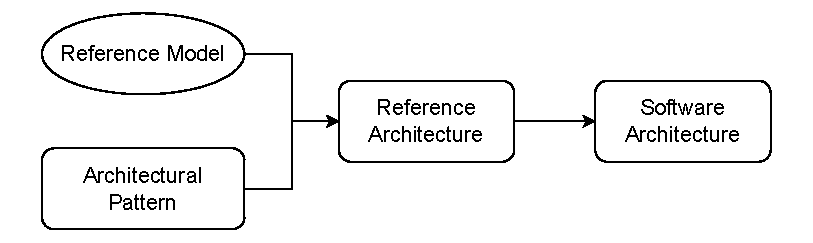
\includegraphics[width=0.8\textwidth]{images/box_and_arrow_sa.drawio.pdf}
    \caption{ارتباط بین مدل‌های مرجع، الگو‌های مربوط به معماری، معماری‌های مرجع
    و معماری‌های نرم‌افزار}
    \label{fig:saStages}
\end{figure}

\subsubsection{\lr{Architectural patterns} یا الگو‌های معماری}

الگو راه‌حلی برای خانواده‌ای از مشکلات می‌باشد. در حقیقت به الگو ممکن است
\lr{Style} هم گفته شود.

وابسته به دامنه کاری نمی‌باشد؛ وقتی در مورد الگوی معماری کلاینت سرور صحبت
می‌کنیم می‌تواند شامل دامنه‌های مختلفی مانند نانوایی تا سیستم‌های بزرگ‌تر شود.

برای مثالی دیگر می‌توان به الگوی \lr{Black board} اشاره کرد که هر آن چیزی که
قرار است خوانده و نوشته شود در این الگو مشخص می‌گردد. از مهم‌ترین کاربرد‌های این
الگو نیز می‌توان به حافظه‌های مشترک در معماری کامپیوتر نیز اشاره کرد.

\subsubsection{\lr{Layering pattern} یا الگو لایه‌بندی کردن}

در روش لایه‌بندی کردن، هر لایه نسبت به لایه‌های دیگر کاملاً متمایز است و زمانی
که نیازمند ایجاد لایه‌ای جدید مانند امنیت هستیم می‌توانیم از این الگو استفاده
کنیم.

برای مثال، لایه‌بندی برای مسئولین یک دانشگاه را در نظر بگیرید، مسئولینی که سمتی
بالایی دارند عموماً در طبقات بالاتر ساختمان دانشگاهی هستند.

\subsubsection{کاربرد الگو}

الگو‌ها روی ویژگی‌های کیفی کار می‌کنند و می‌توان گفت الگو‌ها به طور مستقیم روی
ویژگی‌های کیفی \footnote{\lr{Quality properties}} ارتباط دارند. براساس ویژگی‌های
کیفی، الگو‌ها را انتخاب می‌کنیم. برخی عملکرد مناسب را پوشش می‌دهند و برخی دیگر
امنیت و دسترس‌پذیری بالا را. اگر بخواهیم ویژگی کیفی جدیدی را ایجاد کنیم بایستی
الگو مورد نظر را تغییر دهیم. الگو‌ها عموماً به صورت ترکیبی استفاده می‌شوند.

\begin{itemize}
    \item الگو‌ها تحلیل فضای مسئله را مشخص می‌کنند. در تحلیل سیستم، سیستم را به
    طور واضح خواهیم شناخت. ارتباطات آن را بیشتر می‌توان درک کرد و مشکلی را متوجه
    شد که برای پاسخ به آن در طراحی وارد عمل می‌شویم. تمام نمودار‌ها و
    نیازمندی‌ها در این مرحله مطرح می‌شوند.
    \item طراحی راه‌حل مورد نیاز برای فضای مسئله را بررسی می‌کند. ما نمی‌توانیم
    در فاز طراحی بپرسیم که آیا این کامپوننت با کامپوننت دیگر بایستی ارتباط داشته
    باشد زیرا در فاز فضای مسئله تمام این موارد و ارتباطات بایستی مشخص می‌شد.
\end{itemize}

\subsubsection*{سوال (کنکوری)}

\begin{enumerate}
    \item آیا هر معماری یک طراحی است؟
    \item آیا هر طراحی یک معماری است؟
\end{enumerate}

\subsubsection*{پاسخ سوال اول}

بله هر معماری شامل طراحی می‌باشد که در آن به صورت صریح و مشخص به همراه جزئیات
تمام سیستم مورد بررسی قرار گرفته است و می‌توان از آن‌ها برای پیاده‌سازی محصول
نرم‌افزاری مورد نظر استفاده کرد. همانطور که پیش‌تر گفته شد هر معماری شامل تجرید
کلی از یک سیستم است اما در طراحی ما سطح تجرید را به شدت کم می‌کنیم و در آن وضعیت
المان‌ها، روابط و نمود خارجی آن‌ها را به صورت صریح به همراه جزئیات مطرح می‌کنیم.
پس در هر معماری می‌تواند طراحی وجود داشته باشد.

\subsubsection*{پاسخ به سوال دوم}

خیر هر طراحی یک معماری محسوب نمی‌شود زیرا طراحی به صورت دقیق و با جزئیات کل
سیستم را مورد بررسی قرار می‌دهد اما در معماری سطح تجرید بالا می‌باشد و ما قادر
نخواهیم بود که در آن جزئیات را مطرح کنیم.

\begin{itemize}
    \item گام اول طراحی معماری می‌باشد.
    \item در \lr{RUP} فرایند تشریح اولین قدم می‌باشد.
    \item سند معماری باید به صورت نهایی شده باشد تا بتوان وارد فاز طراحی شد.
    \item سند نیازمندی‌ها نیز باید ۸۰ درصد نیاز‌ها را برآورد و نهایی کرده باشد
    تا بتوان وارد فاز طراحی شد.
\end{itemize}

\subsubsection{\lr{Reference models} یا مدل مرجع}

مدل مرجع تقسیم وظیفه‌مندی یک سیستم همراه با جریان داده آن قسمت می‌باشد.

\begin{itemize}
    \item در مدل مرجع \lr{OSI} هر لایه وظیفه آن به صورت دقیق مطرح شده است.
    \item در امور مالی هیچ وقت انتخاب واحد را انجام نمی‌دهیم.
    \item واحد زمان‌بندی یک \lr{Borker} دارد، یک واحد \lr{Score} و یا واحد
    \lr{Periority}. به طور کل یک پکیج است که تمام موارد گفته شده در آن موجود
    می‌باشد.
\end{itemize}

\subsubsection{\lr{Reference architecture} یا معماری مرجع}

همانطور که از نامش پیداست مانند الگو‌های معماری، اگر بخواهیم سیستم را راه‌اندازی
کنیم که در دامنه آن دقیقاً همان سیستم به شکل دیگر وجود داشته باشد می‌توانیم از
آن سیستم به عنوان مرجع معماری نرم‌افزار خود استفاده کنیم. برای مثال اگر بخواهیم
یک نرم‌افزار دانشگاهی جهت مدیریت دانشجویان بسازیم می‌توانیم از مدل‌های مرجع
دانشگاه‌های دیگر نیز استفاده کنیم.

\subsection*{نکات}

\begin{enumerate}
    \item گام اول طراحی، معماری نیازمندی‌های سطح بالای سیستم است که در همان لحظه
    باید متوجه شویم.
    \item روش تخمین هزینه و زمان انجام کار در معماری مشخص می‌شود.
    \begin{enumerate}
        \item استفاده از روش \lr{COCOMO}: روش کوکومو که از سرکلمات
        \lr{Constructive Cost Model} گرفته شده است در آن میزان تلاش، زمان صرف
        شده و هزینه‌های مربوط به پروژه نرم‌افزاری به صورت کامل برآورد شده است.
        معیار‌های مهم در کوکومو شامل، اندازه پروژه، پیچیدگی انجام پروژه، تجربه
        اعضای تیم و محیط توسعه می‌باشد \cite{COCOMO}.
        \item استفاده از روش \lr{LoC} یا \lr{Line of Code}: این روش هیچ خلاقیتی
        در تخمین هزینه‌ها ندارد ولی یکی از روش‌های اولیه و مبتدیانه برآورد هزینه
        یک پروژه نرم‌افزار براساس تعداد خط کد‌های زده شده می‌باشد.
    \end{enumerate}
    \item در برخی پروژه‌ها گاهی معمار و طراح می‌توانند یک نفر باشند.
    \item یک معمار دائماً ویژگی‌های کیفی را در طراحی و پیاده‌سازی مد نظر دارد.
    \item از یک معماری نرم‌افزاری می‌توانیم اسفاده مجدد کنیم به شرط آن که
    ویژگی‌های کیفی یکسانی داشته باشند.
    \item معماری یک دید ایستا نمی‌باشد.
\end{enumerate}

\subsection{دلیل اهمیت معماری چیست؟}

\begin{enumerate}
    \item معماری نرم‌افزار ارتباطات بین ذینفعان را مشخص می‌کند که هر کدام از
    آن‌ها مجموعه‌ای از نیازمندی‌ها را دارد که حتی بین نیازمندی هر ذینفعی تضادی
    نیز وجود دارد. معماری نرم‌افزار تصمیم اولیه طراحی می‌باشد و تمام ارتباطات را
    به صورت کامل پوشش می‌دهد.
    \item تصمیمات اولیه طراحی: ابتدایی‌ترین نقطه‌ای که می‌توان تصمیم را در آن
    گرفت نیز تحلیل و بررسی می‌شود. \lr{Early design decisions}:
    \begin{enumerate}
        \item معمار قید و بند‌ها را در طراحی تعریف می‌کند.
        \item معمار ساختار سازمانی را به ما دیکته می‌کند.
        \item معمار تسلط کاملی روی ویژگی‌های کیفی دارد.
        \item معمار می‌تواند نیاز‌های آتی را پیشبینی کند.
        \item معمار می‌تواند به آسانی تغییرات را مدیریت کند.
        \item معمار می‌تواند در کامل کردن پروتوتایپ کمک کند.
        \item معمار کسی است که با دقت بیشتر می‌تواند هزینه‌ها و زمانبندی را
        برآورد کند.
    \end{enumerate}
    \item تجرید قابل انتقال از یک سیستم: از سیستم‌های مقیاس بزرگ می‌توان بار‌ها
    استفاده کرد (به عنوان \lr{Reference architecture}). معماری نرم‌افزار یک مدل
    قابل فهم و نسبتاً ساده ایجاد می‌کند تا به وسیله آن مشخص شود چگونه یک سیستم
    ساخته می‌شود و چگونه عناصر آن با یکدیگر کار می‌کنند.
    \item نه فقط کد می‌تواند قابل استفاده مجدد باشد بلکه حتی نیازمندی‌های موجود
    در معماری در مراحل اولیه نیز می‌تواند قابل استفاده مجدد باشد.
    \item عموماً معماری، خط تولید یک معماری مشترک را به اشتراک می‌گذارد.
\end{enumerate}

% در آزمون جامع دکتری پرسش فراوانی دارد.
\subsection{تفاوت معماری سیستم و معماری نرم‌افزار}

در معماری یک نرم‌افزار ملاحضات سیستم نادیده گرفته می‌شود. برای مثال اگر
می‌خواهیم قدرت پردازشی سرور‌ها بیشتر باشد اصلاً در معماری نرم‌افزار آن را مطرح
نمی‌کنیم. در معماری نرم‌افزار در مورد چگونگی ساخت نرم‌افزار از اجزای آن،
ارتباطات و وظایف آن‌ها صحبت می‌کنیم. سرعت‌ها، هزینه‌ها، پهنای باند، ارسال تراکنش
در ثانیه و غیره هیچ وقت در معماری نرم‌افزاری دیده نمی‌شود بلکه در معماری سیستم
تعریف می‌شود. به طور کلی ذهن معمار از کلیه ملاحضات سخت‌افزاری به دور است. زیرا
در سخت افزار نمی‌توانیم قدرت انعطاف‌پذیری که در نرم‌افزار داریم را داشته باشیم
ولی به گونه‌ای است که ویژگی‌های کیفی ما کاملاً با سخت‌افزار در ارتباط می‌باشد.

\subsection{دیدگاه و ساختار یا \lr{View and Structure}}

دیدگاه و ساختار هر دو کاملاً روی یک سکه هستند:

\begin{itemize}
    \item یک دیدگاه نمایشی از مجموعه‌ای منسجم از معماری المان‌ها می‌باشد که شامل
    المان‌ها و روابط بین آن‌ها می‌شود.
    \item یک ساختار مجموعه‌ای از المان‌ها می‌باشد که یا در سخت‌افزار یا در
    نرم‌افزار وجود دارد.
\end{itemize}

\subsection{سه نوع ساختار‌ها}

\subsubsection{\lr{Module} یا ساختار‌های ماژول}

ماژول‌ها یک روش مبتنی بر کد برای بررسی سیستم هستند و به بخش‌های وظیفه‌مندی سیستم
اشاره دارند. این بخش یک دید ثابت دارد. معمولاً سوالات زیر در ماژول‌ها بیان
می‌شود:

\begin{itemize}
    \item \lr{Uses}: در این قسمت مشخص می‌شود که ارتباطات بین عناصر و المان‌ها به
    چه صورتی است.
    \item \lr{Layered}: مشخص می‌شود که هر کدام از المان‌ها در چه لایه‌ای قرار
    می‌گیرند.
    \item \lr{Class}: کلاس‌ها و مدل‌های نرم‌افزاری (موجودیت‌ها) در این قسمت
    تعریف می‌شوند و چون کلاس‌ها به صورت ثابت می‌باشند برخی از اعضای تیم
    نرم‌افزار سه نوع ساختار معماری را ثابت می‌بینند.
    \item \lr{Decomposition}: ماژول‌ها می‌توانند متشکل از چندین زیر ماژول باشند
    که در تمیزی کد و توسعه و دیباگینگ مناسب کمک بسیار زیادی کند. در اینجا مشخص
    می‌شود که چگونه ماژول‌های بزرگ‌تر به ماژول‌های کوچک‌تر جهت مدیریت کد بهتر
    تقسیم می‌شوند.
\end{itemize}

\subsubsection{\lr{Component-and-Connector}}

اجزای این ساختار کامپوننت‌ها در زمان اجرا و اتصال‌هایشان می‌باشد. یک دید پویا
دارد برای تغییرات در حین اجرا.

\begin{itemize}
    \item \lr{Client-Server} نرم‌افزار از چه الگویی استفاده می‌کند.
    \item \lr{Concurrency}: بحث همزمانی تراکنش‌ها و درخواست‌ها در اینجا مطرح
    می‌شود. کدام بخش‌های سیستم می‌توانند به صورت همزمان اجرا شوند؟
    \item \lr{Process}: بحث فرایند‌ها را با استفاده از نمودار‌های \lr{Activity}
    نمایش می‌دهند تا بتوانند فرایند را از صفر تا صد تعریف کنند. چگونه داده‌ها در
    سرتاسر سیستم حرکت می‌کنند؟
    \item \lr{Shared Data}: مخزن داده مشترک اصلی چه چیزی است؟
    \item کدام بخش از سیستم تکرار شده است؟
    \item چگونه می‌توان ساختار سیستم را زمانی که در حال اجرا است تغییر داد؟
\end{itemize}

\subsubsection{\lr{Allocation} یا اختصاص منابع}

\begin{itemize}
    \item \lr{Work assignment}: این ساختار در مورد اختصاص کار‌ها و اسناد مربوط
    به استقرار صحبت می‌کند. اختصاص منابع نرم‌افزاری به سخت‌افزار و برعکس
    می‌باشد.
    \item سند استقرار یا \lr{Deployment document}
    \item سند \lr{Activity} و \lr{Business Processing Model Notation}
    \item \lr{Deployment}: استقرار در حقیقت، تحلیل کارایی، قابلیت دسترس‌پذیری و
    امنیت را مطرح می‌کند.
    \item \lr{Assigned to}: انتساب کار، مدیریت پروژه، استفاده بهتر از تجارب،
    مدیریت بهتر دارایی‌ها
\end{itemize}

نیاز‌های \lr{N-FR} را نمی‌توان خارج از نیاز‌های \lr{FR} سیستم در نظر بگیرم.
نیاز‌های عملیاتی را با استفاده از \lr{Usecase}ها نمایش می‌دهیم که در حقیقت
سناریو‌های سیستم را مطرح می‌کند.

\section{اندازه‌گیری کارایی نرم‌افزار}

\subsection{\lr{Responsiveness} یا پاسخگویی}

در پاسخگویی مطرح می‌شود که یک تسک چقدر سریع می‌تواند توسط یک سیستم تمام شود.
معمولاً با \lr{Waiting time} و \lr{Queue length} می‌توان اندازه‌گیری کرد.

\subsection{\lr{Usage level} یا سطح استفاده}

به چه اندازه‌ای می‌توانیم به صورت مناسب و مطلوب از المان‌های مختلف در سیستممان
استفاده کنیم. معیار‌های اندازه‌گیری آن \lr{Throughput} یا گذردهی و
\lr{Utilization} می‌باشد.

\subsection{\lr{Waiting time}}

مدت زمان بین رسیدن تسک به سرویس و شروع ارائه سرویس به آن تسک (درخواست) را
می‌گویند.

\subsection{\lr{Queue length}}

تعداد تسک‌ها (درخواست‌ها) در صف انتظار برای سرویس‌گیری.

\subsection{\lr{Task length or Service time}}

به هر درخواست درون صف چقدر طول می‌کشد که سرویس‌دهی انجام شود. عموماً وابسته به
میزان پردازشی سرور و محاسبه درخواست می‌باشد.

\subsection{\lr{Utilization}}

مدت زمانی که یک قطعه از تجهیزات در حال استفاده است نسبت به کل زمان استفاده از
آن، محاسبه می‌شود.

\subsection{\lr{Throughput}}

نرخ کامل شدن تسک‌ها در سیستم می‌باشد.

\subsection{\lr{Good-put}}

داده‌ای است که باز ارسال نشده باشد. یک بسته سالم بدون هیچ باز ارسالی از سمت مبدا
به سمت مقصد را گویند.

\subsection{\lr{Missionability} یا ماموریت‌پذیری}

ماموریت‌پذیری نشان می‌دهد که سیستم مورد نظر در آن بازه زمانی که عملیاتی را انجام
می‌داده است چقدر رضایت در کارایی و گذردهی داشته است. چقدر در آن زمانی که در
دسترس بوده است تسک‌هایی را رد کرده و تسک‌هایی را با موفقیت انجام داده است.

\subsection{\lr{Dependability}}

این اندازه‌گیری مشخص می‌کند که چقدر یک سیستم در طول اجرا قابل اطمینان می‌باشد.
فرمول‌هایی را مطرح می‌کند که همگی از نوع زمان هستند. نکته آن است که تعداد
شکست‌ها در سیستم باید کم باشد و همچنین زمانی که در وضعیت شکست قرار داریم بایستی
سریع ریکاوری انجام شود تا دوباره سیستم به حالت صحیح قبلی خود بازگردد.

ابزار‌های اندازه‌گیری آن عبارت‌اند از:

\begin{itemize}
    \item \lr{Number of failures per day}
    \item \lr{MTTF (Mean Time to Failure)}
    \item \lr{MTTR (Mean Time to Recovery or Repair)}
    \item \lr{Long Term Availability}
    \item \lr{Cost of Failure}
\end{itemize}

\subsection{\lr{Productivity} یا معیار بهره‌وری}

این معیار مشخص می‌کند که یک کاربر چقدر بهینه می‌تواند کار خود را با محصول مورد
نظر انجام دهد.

ابزار‌های اندازه‌گیری آن عبارت‌اند از:

\begin{itemize}
    \item \lr{User Friendliness}
    \item \lr{Understandability}
\end{itemize}

برای مثال، \lr{User Interface (UI)} یک اپلیکیشن موبایل چقدر خوب طراحی شده است که
کاربر می‌تواند در سریع‌ترین حالت ممکن گزینه‌های مدنظر خود را پیدا کند؟

\subsection{دسترس‌پذیری، قابلیت اعتماد و قابلیت اطمینان}

\subsubsection{\lr{Mean Time Between Failures (MTBF)}}

زمان سپری شده پیشبینی شده بین خرابی‌های یک سیستم در حین کار است. \lr{MTBF}
می‌تواند زمان بین خرابی‌های یک سیستم را محاسبه کند.

\begin{LTR}
    MTBF Defined as: total time in service / number of failures
\end{LTR}

\begin{equation}
    MTBF = \frac{\sum(X - Y)}{Z}
\end{equation}

\begin{itemize}
    \item \lr{X}: \lr{Start of downtime}
    \item \lr{Y}: \lr{Start of uptime}
    \item \lr{Z}: \lr{Number of failures}
\end{itemize}

\begin{figure}[H]
    \centering
    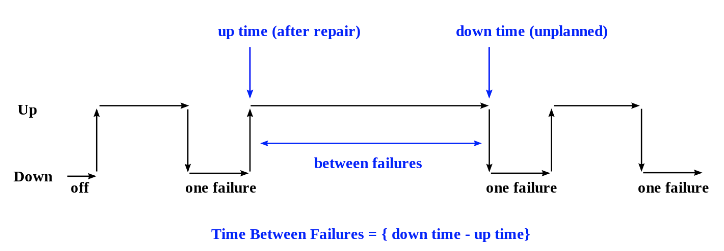
\includegraphics[width=0.9\textwidth]{images/mtbf.png}
    \caption{\lr{Mean Time Between Failures (MTBF)}}
    \label{fig:MTBFDiagram}
\end{figure}

\subsubsection{\lr{Mean Time to Failures (MTTF)}}

طول زمانی که انتظار داریم یک دستگاه یا هر چیزی در مدار باقی بماند. \lr{MTTF}
معیاری است که در سخت‌افزار استفاده می‌شود. مدت زمانی که انتظار داریم یک دستگاه
یا محصول کار کند. \lr{MTTF} یکی از هزاران راه‌یی است که می‌توان قابلیت اعتماد و
پایداری سخت‌افزار یا بقیه تکنولوژی‌ها را با آن اندازه‌گیری کرد.

\subsubsection{\lr{Mean Time to Repair or Recovery (MTTR)}}

مدت زمانی که طول می‌کشد تا سیستم به مدار برگردد. یا به عبارتی دیگر میانگین زمانی
که نیاز است تا یک کامپوننت شکست خورده تعمیر و ریکاوری شود.

\subsubsection{تفاوت میان \lr{MTTF} و \lr{MTBF}}

\begin{itemize}
    \item معیار \lr{MTBF} برای محصولاتی است که می‌توان آن‌ها را در حین خرابی
    تعمیر کرد تا سریعاً به مدار بازگردد.
    \item معیار \lr{MTTF} برای محصولاتی که قابل تعمیر نیستند استفاده می‌شود.
    زمانی از این معیار استفاده می‌کنیم که به دنبال تعمیرپذیری محصول نباشیم.
\end{itemize}

\subsection*{نکته}

\begin{itemize}
    \item بازه‌های زمانی بررسی سیستم در سازمان بایستی به صورت مشخص باشد (ساعتی،
    روزانه، هفتگی، ماهانه، سالانه).
    \item یک قطعه (دستگاه، نرم‌افزار و هر چیزی) می‌تواند \lr{Available} باشد ولی
    \lr{Reliable} نباشد.
    \item نرخ خرابی: $\frac{Number Of Failures}{Total Time In Service}$
\end{itemize}

\section{دسترس‌پذیری}

دسترس‌پذیری یا \lr{Availability}  یعنی زمانی که می‌خواهیم از چیز استفاده کنیم و
آن چیز بایستی ارائه سرویس را انجام دهد.

\begin{equation}
    Availability = \frac{uptime}{Total Service Time}
\end{equation}

\subsection*{مثال}

یک ماشین هر یک ساعت، ۶ دقیقه داون است. مطلوب است محاسبه \lr{Availability} و
\lr{Reliability}:

\begin{equation}
    Uptime = 60-6 = 54
\end{equation}

\begin{equation}
    Availability = \frac{Uptime}{Total Service Time} = \frac{54}{60} = 0.9 or 90\%
\end{equation}

برای محاسبه قابلیت اطمینان می‌توان گفت که وقتی در یک ساعت ۶ دقیقی با قطع کارکرد
خودرو همراه هستیم، پس قابلیت اطمینان زیر یک ساعت یا کمتر از ۵۴ دقیقه است.

\subsection{بازه زمانی یا \lr{Total time}}

در دسترس‌پیذیرپذیری بررسی \lr{Total time} بسیار مهم است، چرا که سرویس در آن زمان
بایستی بدون مشکل در دسترس باشد و به صورت صحیح تا انتهای بازه مشخص \lr{Total
time} به کار خودش ادامه دهد. برای مثال سیستم آموزشیار بایستی در ابتدای ترم جهت
اخذ واحد درسی دانشجویان، در یک بازه یک ماهه به طور مثال کاملاً در دسترس و قابل
اطمینان باشد. اما با تغییر دامنه از سیستم انتخاب واحد دانشگاه به دامنه بانکی این
گفته صادق نیست، زیرا محصولات و سرویس‌‌های بانکی بایستی ۲۴ ساعته ۷ روز هفته در
دسترس باشند و کاملاً قابلیت اطمینان را به همراه داشته باشند.

\subsection{ارتباط میان \lr{Availability} با \lr{Reliability}}

عموماً وقتی سیستمی \lr{Reliable} است یعنی دارای \lr{Availability} بالایی است اما
وقتی سیستمی \lr{Available} است ممکن است آن سیستم قابل اطمینان باشد و ممکن است
قابل اطمینان نباشد. زمانی کاملاً قابل اطمینان است که تمام آن سیستم با آزمون‌ها و
ارزیابی‌ها پوشش داده شده باشد و فاقد هر گونه \lr{Fault} باشد و از سمتی در هنگام
استقرار نیز تمام نکات \lr{Availability} به عنوان ویژگی کیفی رعایت و پیاده‌سازی
شده باشند. به این صورت هم دسترس‌پذیری بالایی خواهد داشت هم از قابلیت اطمینان
بالایی برخوردار خواهد بود.

\subsection*{نکته}

در قابلیت اطمینان وابستگی به موقعیت می‌تواند عامل مشخص‌کننده‌ای باشد. برای مثال
با استفاده از یک موتور شارژی می‌توان درون شهر فعالیت کرد، اما با همان موتور
شارژی نمی‌توان به جنوب کشور سفر کرد.

\subsection{\lr{Mean Down Time (MDT)}}

میانگین زمانی که یک سیستم قابل استفاده نباشد. \lr{MDT} با فاکتور‌های زیر همراه
است:

\begin{itemize}
    \item \lr{System failure}:
    \begin{itemize}
        \item سیستم به طور کلی فاقد هر گونه \lr{Fault} باشد.
        \item منتظر تامین قطعات نباشد
        \item سیستم نیاز به تعمیر داشته باشد.
    \end{itemize}
    \item \lr{Scheduled downtime}:
    \begin{itemize}
        \item نگهداری پیشگیرانه
        \item به روزرسانی سیستم
        \item کالیبراسیون
        \item سایر اقدامات اداری (\lr{Administrative})
    \end{itemize}
\end{itemize}

مقدار \lr{MDT} هر چقدر کمتر باشد دسترس‌پذیری نیز بیشتر خواهد بود.

\subsection{بدست آوردن مدت زمان \lr{Down time}}

برای محاسبه مدت زمان قطع سرویس یک سیستم از فرمول زیر استفاده کنیم:

\begin{equation}
    (Availability - 1) * Total Time = DownTime
\end{equation}

اگر یک سیستم در یک سال $99.99\%$ دسترس‌پذیری داشته باشد چند دقیقه \lr{Down time}
خواهد داشت:

\begin{equation}
    (0.9999 - 1) * 365D = Down Time
\end{equation}

\begin{equation}
    (0.0001) * 8760Hr = 0.876Hr
\end{equation}

\begin{equation}
    0.876Hr \rightarrow 52.56Min
\end{equation}

\begin{equation}
    52.56Min \rightarrow 52 Min \rightarrow 0.56Min
\end{equation}

در نهایت پاسخ ۵۲ دقیقه و ۳۴ ثانیه قطعی سرویس با $99.99\%$ دسترس‌پذیری می‌باشد.

\newpage
\bibliographystyle{unsrt-fa}
\bibliography{refs.bib}
\end{document}